\documentclass[12pt,a4paper,oneside]{report} % Document class and options
\usepackage[utf8]{inputenc} % Input encoding
%\usepackage[english]{babel} % Language package (commented out)
\usepackage[T1]{fontenc} % Font encoding
\usepackage{amsmath} % Math package
\usepackage{amsfonts} % Math fonts
\usepackage{amssymb} % Math symbols
\usepackage{makeidx} % Indexing
\usepackage{graphicx} % Graphics package
\usepackage[margin=1in]{geometry} % Page margins
\graphicspath{{images/}} % Path to images
\usepackage{times} % Times font
\usepackage{nomencl} % Nomenclature package
%\usepackage{appendix} % Appendix package (commented out)
\usepackage[round]{natbib} % Bibliography package
\usepackage[toc,page]{appendix} % Appendix package with TOC and page options
\usepackage{setspace} % Line spacing
\usepackage{color} % Color package
\usepackage{fancybox} % Fancy boxes
\usepackage{lipsum} % Lorem ipsum text
\usepackage{tocloft} % TOC customization
\usepackage[bookmarks = true]{hyperref} % Hyperlinks
\usepackage{caption} % Captions
\usepackage{subcaption} % Sub-captions
\usepackage{amsmath} % Math package (duplicate)
\usepackage{enumitem} % Enumerations
\usepackage{lscape} % Landscape pages
\usepackage{ulem} % Underlining text
\usepackage{longtable} % Long tables
\usepackage{datetime} % Custom date formats

%\usepackage{emptypage} %removes fancy headers from blank page
%\usepackage[nottoc]{tocbibind} %adds ref and ind in toc
%\usepackage[toc,page]{appendix} %creats a new page for appendices title





% Abbreviations
\usepackage{acro} % Abbreviations package
\DeclareAcronym{usa}{ % Declare acronym for USA
    short=USA, % Short form
    long=United States of America, % Long form
}
\DeclareAcronym{eu}{ % Declare acronym for EU
    short=EU, % Short form
    long=European Union, % Long form
}
\DeclareAcronym{ussr}{ % Declare acronym for USSR
    short=USSR, % Short form
    long=Union of Soviet Socialist Republics, % Long form
}
% Call method\ac{usa}
% Symbols
\usepackage[symbols,nogroupskip,nonumberlist,sort=use]{glossaries-extra} % Symbols package
\makenoidxglossaries % Create glossaries

\glsxtrnewsymbol[description={position}]{x}{\ensuremath{x}} % Define symbol for position
\glsxtrnewsymbol[description={velocity}]{v}{\ensuremath{v}} % Define symbol for velocity
\glsxtrnewsymbol[description={acceleration}]{a}{\ensuremath{a}} % Define symbol for acceleration
\glsxtrnewsymbol[description={time}]{t}{\ensuremath{t}} % Define symbol for time
\glsxtrnewsymbol[description={force}]{F}{\ensuremath{F}} % Define symbol for force
% Call method $\gls{F}$
% Date format
\newdateformat{monthyear}{\monthname[\THEMONTH], \THEYEAR} % Custom date format
% Page style
\usepackage{fancyhdr} % Fancy headers and footers
\pagestyle{fancy} % Set page style to fancy
\fancyhf{} % Clear all header and footer fields
\fancyhead[LE, RO]{\thepage} % Page number in header
\fancyhead[RE]{\it{\nouppercase{\leftmark}}} % Left header
\fancyhead[LO]{\it{\nouppercase{\rightmark}}} % Right header
\fancyfoot[C]{\thepage} % Centered page numbers at the bottom
% Nomenclature command
\newcommand{\nm}[2]{\nomenclature{#1}{#2}} % Define nomenclature command
% TOC and bibliography names
\renewcommand{\contentsname}{Table of Contents} % Rename TOC
\renewcommand{\bibname}{References} % Rename bibliography
%\renewcommand{\nomname}{List of Abbreviations}
% Document metadata
\author{SUBHAM KUMAR} % Author name
\title{PHD THESIS} % Title
% Margin settings
\geometry{
    paper=a4paper, % A4 paper size
    left=35mm, % Left margin
    right=25mm, % Right margin
    top=25mm, % Top margin
    bottom=25mm, % Bottom margin
    bindingoffset=5mm % Binding offset
}
% Chapter/section headings
\usepackage{sectsty} % Section styling
% Avoid redefining \chapterfont if it's already defined
\providecommand{\chapterfont}{\relax}
\providecommand{\sectionfont}{\relax}
\providecommand{\subsectionfont}{\relax}
\providecommand{\subsubsectionfont}{\relax}
\chapterfont{\fontsize{16pt}{18pt}\selectfont\bfseries} % Chapter number
\sectionfont{\fontsize{14pt}{16pt}\selectfont\bfseries} % Chapter title heads
\subsectionfont{\fontsize{12pt}{14pt}\selectfont\bfseries} % Section headings
\subsubsectionfont{\fontsize{12pt}{14pt}\selectfont\bfseries} % Subsection headings
% Additional packages
\usepackage{ragged2e} % Ragged text
\usepackage{lscape} % Landscape pages
\usepackage{booktabs} % Booktabs for tables
\usepackage{graphicx} % Graphics package
\usepackage{float} % Floating objects



\usepackage{titlesec} % Required for \titleformat
% Customize chapter heading format 
\titleformat{\chapter}[display] 
{\normalfont\bfseries  \fontsize{18pt}{20pt}\selectfont} % Text format for the chapter heading 
{\centering Chapter \thechapter} % Format for the chapter number 
{20pt} % Space between number and title 
{\fontsize{16pt}{20pt}\selectfont}% Font size for the chapter title
%\usepackage{quotchap}

%\titleformat{name=\chapter,numberless}[block] {\normalfont\huge\filcenter\bfseries}{}{0pt}{\huge}[\addcontentsline{toc}{chapter}{\chaptertitle}]
\titleformat{name=\chapter,numberless}[block] {\normalfont\centering \bfseries}{}{0pt}{\fontsize{16pt}{10pt}\selectfont}

\setcounter{secnumdepth}{3}
\setcounter{tocdepth}{3}

\usepackage{Edit} % Edit package
\raggedbottom % Ragged bottom
\includeonly{
    Frontmatter/Cover, % Cover page
    Frontmatter/InnerCover, % Inner cover page
    Frontmatter/SelfDeclarationCertResScholar, % Declaration certificate
    Frontmatter/CertSupervisor, % Supervisor certificate
    Frontmatter/CopyrightTranCert, % Copyright transfer certificate
    Frontmatter/Ackowledgments, % Acknowledgments
    mainmatter/c1, % Chapter 1
    mainmatter/c2, % Chapter 2
    mainmatter/c3, % Chapter 3
    mainmatter/c4, % Chapter 4
    mainmatter/c5, % Chapter 5
    mainmatter/c6, % Chapter 6
    backmatter/app1, % Appendix 1
    backmatter/app2, % Appendix 2
    backmatter/pub % Publications
}
% Cover page
\begin{document}
\pagenumbering{roman} % Roman page numbering for front matter
\pagestyle{plain}
\onehalfspacing % Front matter
\begin{titlepage} 
\centering 
% TITLE OF THE THESIS 
{\fontfamily{pbk}\selectfont\textbf{\fontsize{18pt}{20pt}\selectfont \Titel}}\\[1cm] 

% University Logo (replace 'university_logo.png' with your logo file) 
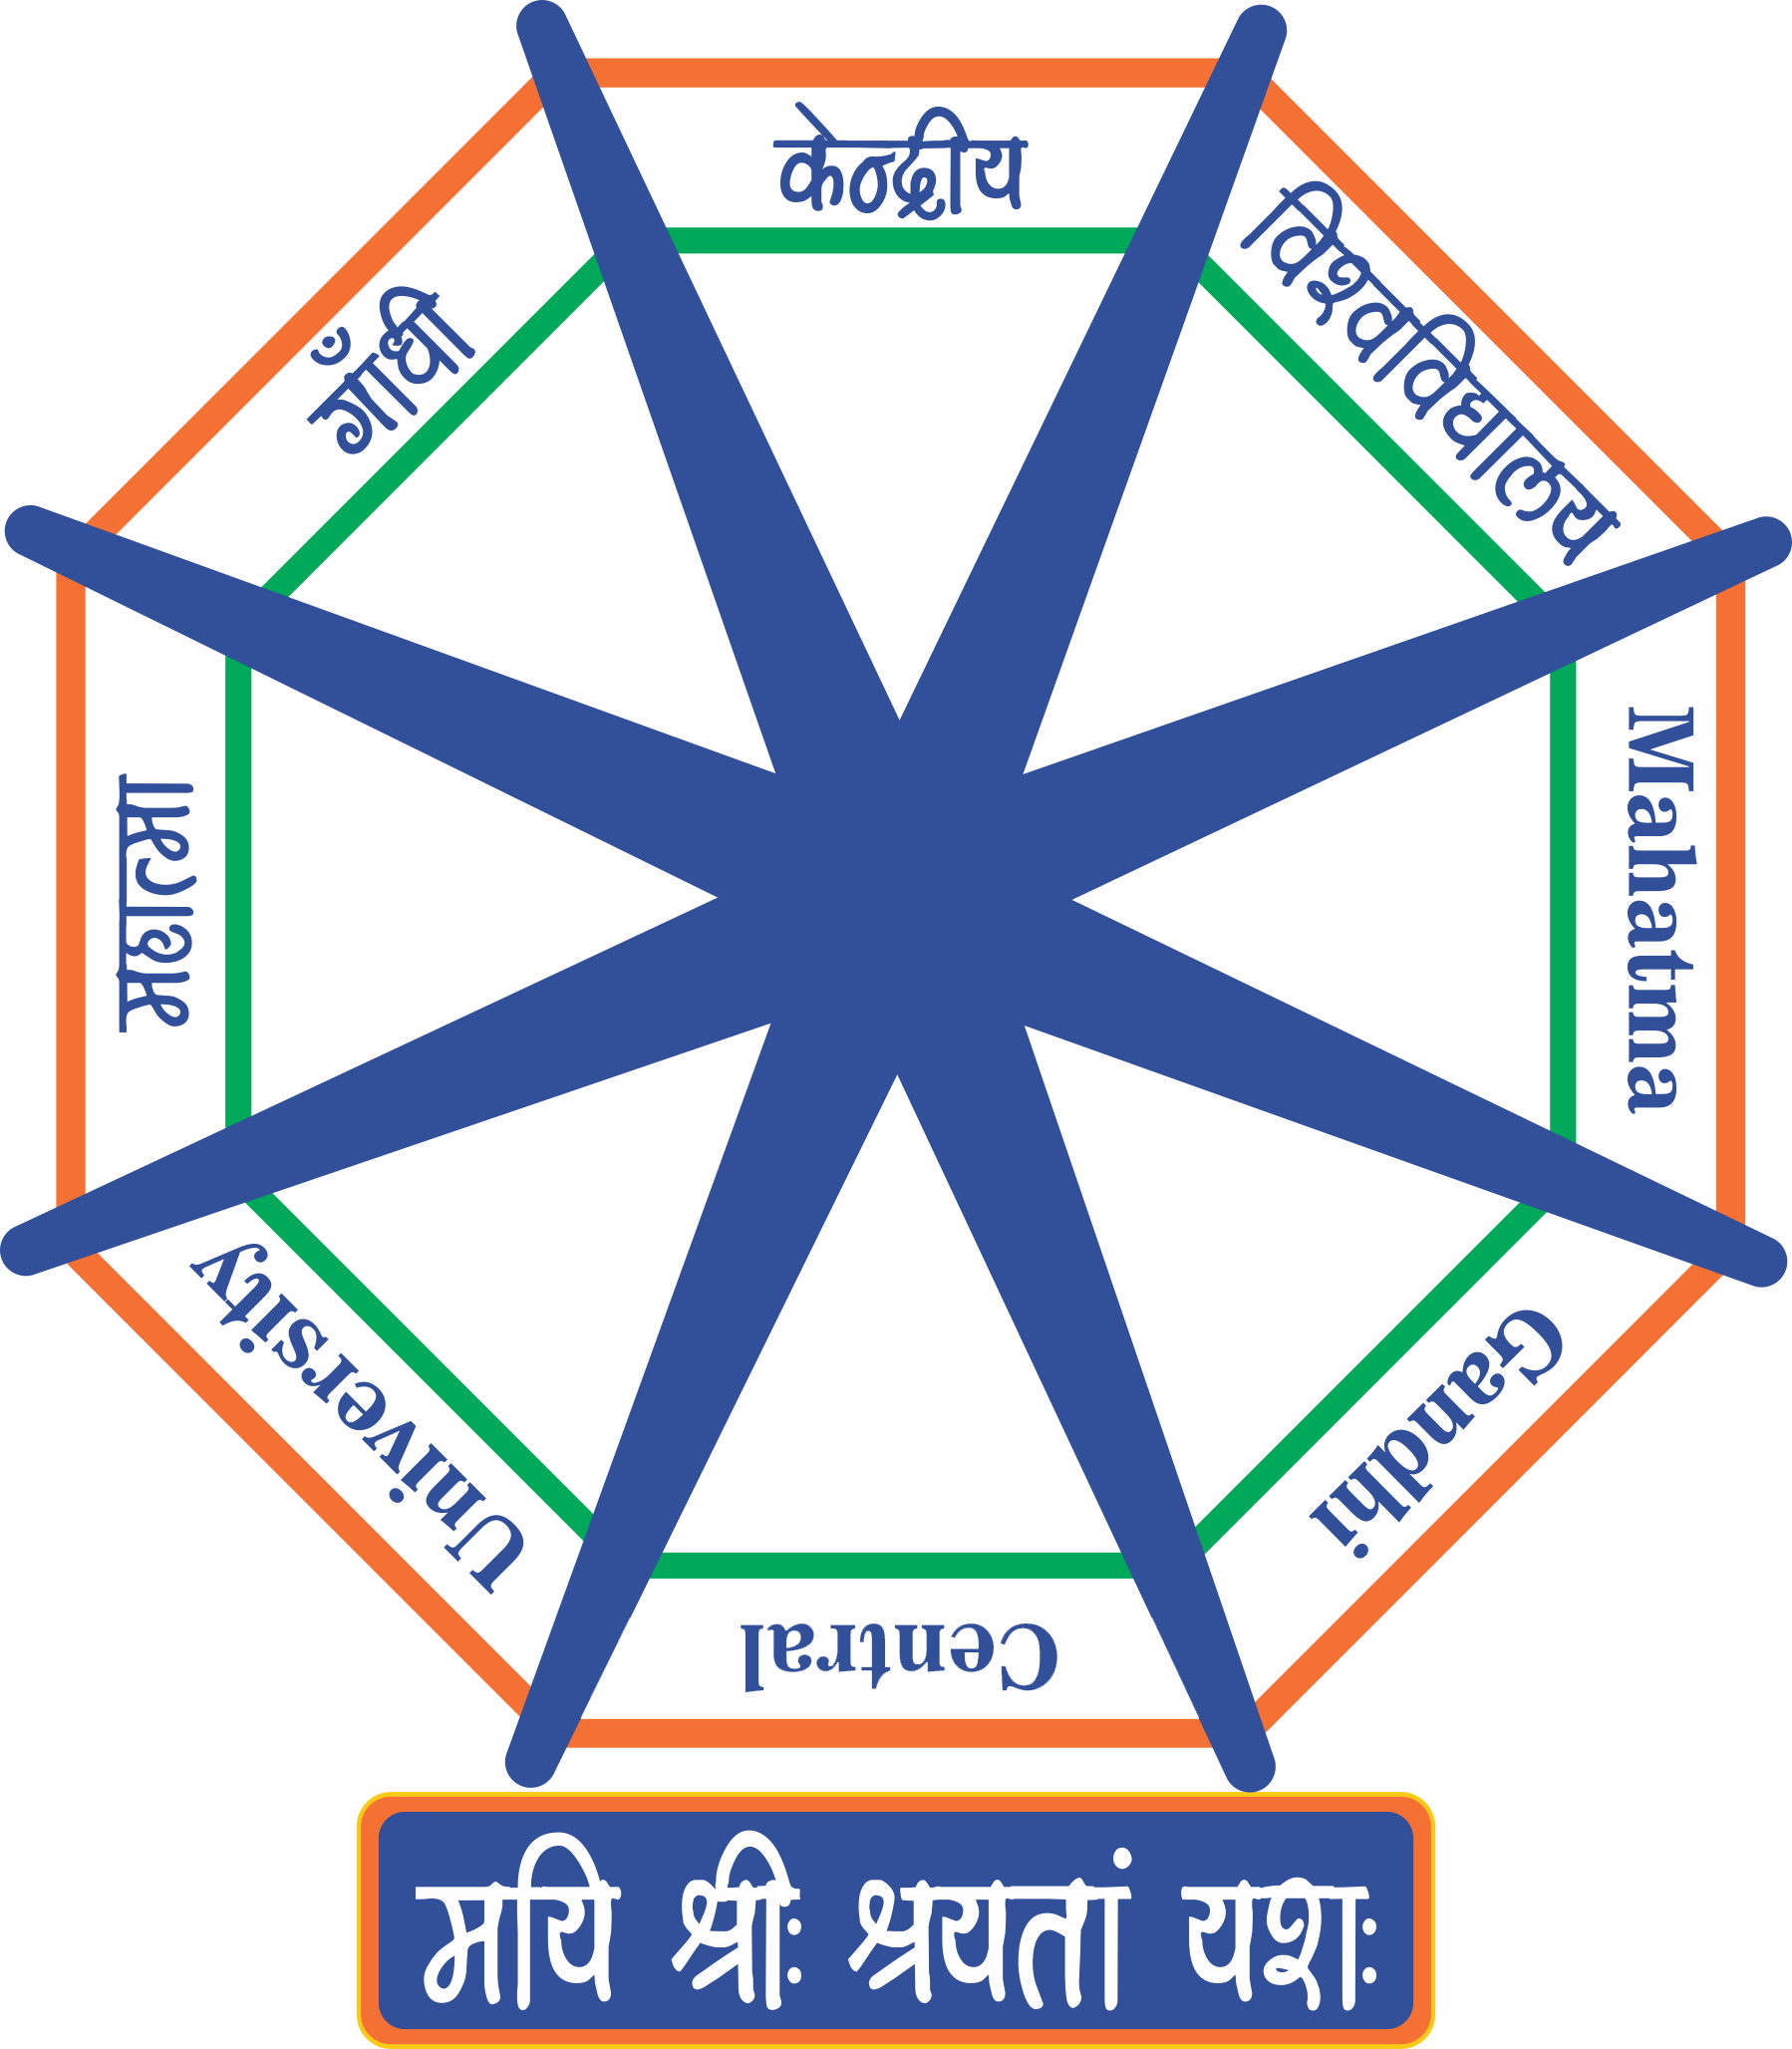
\includegraphics[width=0.2\textwidth]{mgcu}\\[.75cm]

% Thesis submitted in partial fulfilment 
{\fontsize{14}{16}\selectfont Thesis submitted in partial fulfilment}\\ 
{\fontsize{14}{16}\selectfont for the Award of}\\[.5cm] 
% DOCTOR OF PHILOSOPHY 
{\fontsize{16}{18}\selectfont\textbf{\Digree}}\\[0.5cm] 
% in 
{\fontsize{14}{16}\selectfont{in}}\\[0.5cm] 
% Subject 
{\fontsize{16}{18}\selectfont\textbf{\subject}}\\[0.5cm] 
% By 
{\fontsize{14}{16}\selectfont{By}}\\[0.5cm] 
{\fontsize{16}{18}\selectfont\textbf{\Author}}\\[1cm] 
% Under the supervision of 
{\fontsize{14}{16}\selectfont Under the supervision of}\\[0.5cm] 
{\fontsize{14}{16}\selectfont\textbf{\Supervisor}}\\[1cm] 
% DEPARTMENT OF .. 
{\fontsize{14}{16}\selectfont\textbf{\Department}}\\[0.5cm]
 % SCHOOL OF 
{\fontsize{14}{16}\selectfont\textbf{\School}}\\[1cm] 
% MAHATMA GANDHI CENTRAL UNIVERSITY 
{\fontsize{14}{16}\selectfont\textbf{\UniName}}\\[0.5cm]
{\fontsize{14}{16}\selectfont \UniAddress}\\[1cm]

\begin{table}[h]
\begin{center}
\begin{tabular}{r  l}
   \begin{minipage}{0.45\textwidth}
\begin{flushleft}
\begin{center}
% Month, Year(First submission date) 
{\fontsize{14}{16}\selectfont \FSDate}
% Month, Year (First submission date) 
%{\fontsize{14}{16}\selectfont\monthyear\today}\\[1cm]
\end{center}
\end{flushleft}
\end{minipage}
&
\begin{minipage}{0.45\textwidth}
\begin{flushleft}
\begin{center}
% ENROLMENT NUMBER 
{\fontsize{14}{16}\selectfont \Enrolment} 
\end{center}
\end{flushleft}
\end{minipage}
\noindent
\\
\end{tabular}
%\label{tab1}
\end{center}
\end{table}
\end{titlepage} % Cover page
\begin{titlepage} 
\centering 
% TITLE OF THE THESIS 
{\fontfamily{pbk}\selectfont\textbf{\fontsize{18pt}{20pt}\selectfont \Titel}}\\[1cm] 

% University Logo (replace 'university_logo.png' with your logo file) 
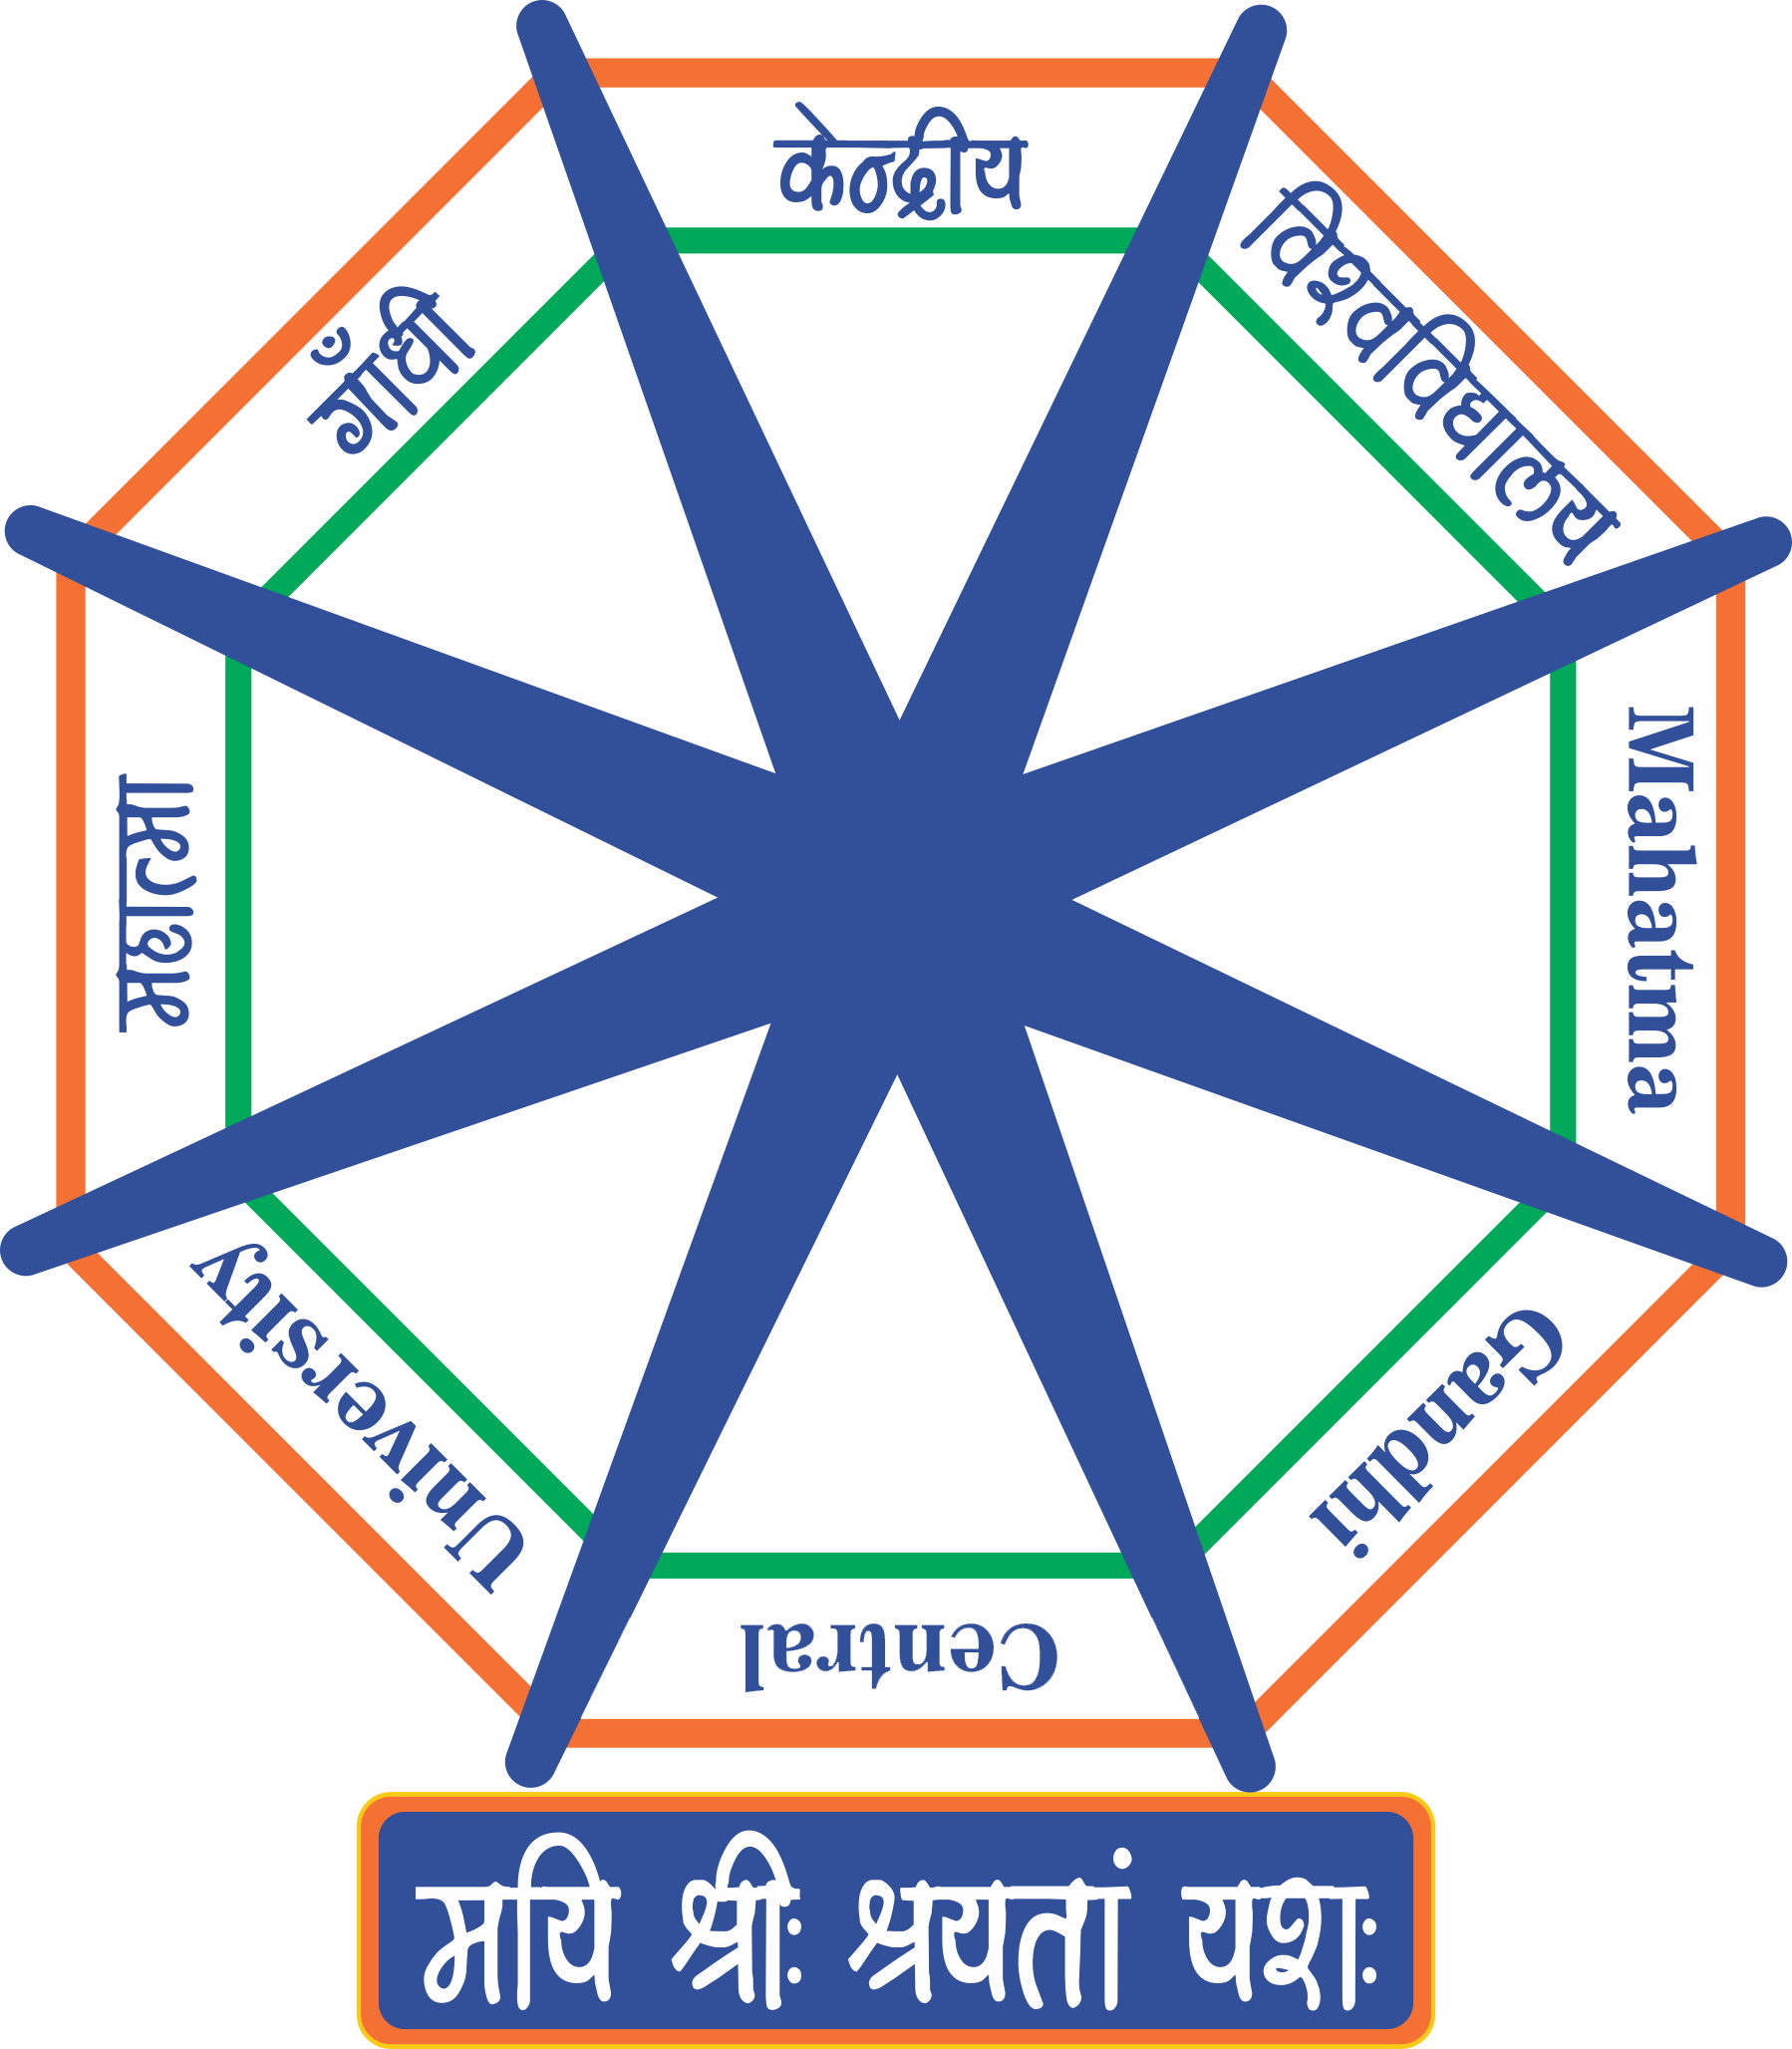
\includegraphics[width=0.2\textwidth]{mgcu}\\[.75cm]

% Thesis submitted in partial fulfilment 
{\fontsize{14}{16}\selectfont Thesis submitted in partial fulfilment}\\ 
{\fontsize{14}{16}\selectfont for the Award of}\\[.5cm] 
% DOCTOR OF PHILOSOPHY 
{\fontsize{16}{18}\selectfont\textbf{\Digree}}\\[0.5cm] 
% in 
{\fontsize{14}{16}\selectfont{in}}\\[0.5cm] 
% Subject 
{\fontsize{16}{18}\selectfont\textbf{\subject}}\\[0.5cm] 
% By 
{\fontsize{14}{16}\selectfont{By}}\\[0.5cm] 
{\fontsize{16}{18}\selectfont\textbf{\Author}}\\[1cm] 
% Under the supervision of 
{\fontsize{14}{16}\selectfont Under the supervision of}\\[0.5cm] 
{\fontsize{14}{16}\selectfont\textbf{\Supervisor}}\\[1cm] 
% DEPARTMENT OF .. 
{\fontsize{14}{16}\selectfont\textbf{\Department}}\\[0.5cm]
 % SCHOOL OF 
{\fontsize{14}{16}\selectfont\textbf{\School}}\\[1cm] 
% MAHATMA GANDHI CENTRAL UNIVERSITY 
{\fontsize{14}{16}\selectfont\textbf{\UniName}}\\[0.5cm]
{\fontsize{14}{16}\selectfont \UniAddress}\\[1cm]

\begin{table}[h]
\begin{center}
\begin{tabular}{r  l}
   \begin{minipage}{0.45\textwidth}
\begin{flushleft}
\begin{center}
% Month, Year(First submission date) 
{\fontsize{14}{16}\selectfont \FSDate}
% Month, Year (First submission date) 
%{\fontsize{14}{16}\selectfont\monthyear\today}\\[1cm]
\end{center}
\end{flushleft}
\end{minipage}
&
\begin{minipage}{0.45\textwidth}
\begin{flushleft}
\begin{center}
% ENROLMENT NUMBER 
{\fontsize{14}{16}\selectfont \Enrolment} 
\end{center}
\end{flushleft}
\end{minipage}
\noindent
\\
\end{tabular}
%\label{tab1}
\end{center}
\end{table}
\end{titlepage} % Inner cover page
\clearpage \phantomsection \addcontentsline{toc}{chapter}{Declaration Certificate} % Add to TOC
\chapter*{\uline{Declaration by Research Scholar}}

\justifying 
I, \sAuthor \  certify that the work embodied in this \sDigree \  thesis is my own bonafide work carried out by me under the supervision of \Supervisor \ and the co-supervision of  \CoSupervisor  \ for a period of \superDuration \ from \FsDate \ to \LsDate \ at \sUniName \ and \uline{(Name of the Institution where work has been carried out partly or fully)}. The matter embodied in this \sDigree \ thesis has not been submitted for the award of any other degree/diploma.
\par I declare that I have faithfully acknowledged, given credit to, and referred to the research workers wherever their works have been cited in the text and the body of the thesis. I further certify that I have not willfully lifted up someone else's work, para, text, data, results, etc., reported in journals, books, magazines, reports, dissertations, theses, etc., or available at websites, and included them in this \sDigree \ thesis and cited as my own work.\\ 
\vspace{1.5cm} 

\begin{table}[h]
\begin{center}
\begin{tabular}{r  l}
   \begin{minipage}{0.45\textwidth}
\begin{flushleft}
\raggedright 
Date: \Date\\ 
Place: \Place\\ 
\end{flushleft}
\end{minipage}
&
\begin{minipage}{0.45\textwidth}
\begin{flushleft}
\raggedleft 
\textbf{(Signature of the Scholar)}\\ 
\textbf{(\sAuthor)}\\ 
\end{flushleft}
\end{minipage}
\noindent
\\
\end{tabular}
%\label{tab1}
\end{center}
\end{table}
 % Declaration certificate
\clearpage \phantomsection \addcontentsline{toc}{chapter}{Supervisor Certificate} % Add to TOC
\chapter*{\uline{Certificate by Supervisor}}
\justifying 
This is to certify that the thesis entitled "\textbf{ \Titel \ } "
is original work and has been carried out by Mr/Ms \sAuthor \ Enrolment No. \Enrolment \ under my guidance and supervision for the degree of \textbf{ \sdigree } in \uline{.......................} to be awarded by Mahatma Gandhi Central University, Bihar.\\
To the best of my knowledge and belief this thesis
\begin{enumerate}[label=\roman*.]
\item 
embodies the work of research scholar himself / herself,
\item
has duly been completed,
\item
fulfils the requirements of the ordinance related to Ph.D. degree of the University.
\item
contents of the thesis do not form the basis for the award of any other degree/diploma or
similar title to the research scholar or to anybody else from this or any other
University/lnstitution.
\end{enumerate}
\vspace{1.5cm} 

\begin{table}[h]
\begin{center}
\begin{tabular}{r  l}
   \begin{minipage}{0.45\textwidth}
\begin{flushleft}

\raggedright 
\begin{center}
(Co-supervisor's signature,name and Designation)\\ 
\end{center}

\end{flushleft}
\end{minipage}
&
\begin{minipage}{0.45\textwidth}
\begin{flushleft}
\raggedleft 
\begin{center}
(Supervisor's signature,name and Designation)\\ 
\end{center}
\end{flushleft}
\end{minipage}
\noindent
\\
\end{tabular}
%\label{tab1}
\end{center}
\end{table}
 % Supervisor certificate
\clearpage \phantomsection \addcontentsline{toc}{chapter}{Copyright Transfer Certificate} % Add to TOC
\chapter*{\uline{Copyright Transfer Certificate}}

\textbf{Title of the Thesis:} \Titel \\[.5cm]
\textbf{Name of Research Scholar:} \sAuthor \\[1cm]

\centering
\textbf{Copyright Transfer}\\[.5cm]
\justifying 
The undersigned hereby assigns to the Mahatma Gandhi Central University all rights under copyright that may exist in and for the above thesis submitted for the award of the Ph.D. degree.
\vspace{1.25cm} 

\begin{table}[h]
\begin{center}
\begin{tabular}{r  l}
   \begin{minipage}{0.45\textwidth}
\begin{flushleft}
\raggedright 
\end{flushleft}
\end{minipage}
&
\begin{minipage}{0.45\textwidth}
\begin{flushleft}
\raggedleft 
\begin{center}
\textbf{Signature of the Scholar}\\ 
\end{center}
\end{flushleft}
\end{minipage}
\noindent
\\
\end{tabular}
%\label{tab1}
\end{center}
\end{table}
\vspace{1.25cm} 
\justifying 
Note: However, the author may reproduce or authorize others to reproduce material extracted verbatim from the thesis or derivative Of the thesis for author's personal use provided that the source and the University's copyright notice are indicated.

 % Copyright transfer certificate
\clearpage \phantomsection \addcontentsline{toc}{chapter}{Ackowledgment} % Add to TOC
\chapter*{\centering \uline{Acknowledgment}}

%\justifying 

This M.Tech \textbf{ReportType} is the result of hard work, upon which many people have contributed and given their support. I
have made this dissertation on the topic \textbf{"ReportTitel ."} I have also tried my best in this dissertation to
explain all the related detail. I would like to express my sincere gratitude towards my Superviser \textbf{Supervisor}, Department of \textbf{Department}, for providing excellent guidance, encouragement, inspiration, and constant and
timely support throughout this \textbf{Degree}  dissertation work. He taught me how to pursue the right aim towards the work, and showed me differnt ways to approach the research problem. His wide knowledge and logical ways of thinking have been great value for me, and his understanding and guidance have provided the successful completion of the
Dissertation work.

First and foremost, I would like to express my gratitude to our beloved Dean of the Computational Sciences,
Information and Communication Technology and Head of Department of Computer Science and Information Technology \textbf{HodName},
for providing his kind support in various aspects. A special thanks to all the Respected Teachers of the Department of Computer Science and Information Technology.

I am always grateful to the university, our Hon’ble Vice chancellor \textbf{Vc} for providing
such a good research environment.

	Special thanks to Ph.D scholar, especially \textbf{Ritika Singh}, \textbf{Surbhi Kumari}, \textbf{Ibrahim Momin},
\textbf{Naushad Ahmad} and  my friends \textbf{Tej Prakash}, \textbf{Gajendra Patel}, \textbf{Abhijeet Kumar},
\textbf{Amod Kumar}, \textbf{Rana Kumar}, \textbf{Krishna Murari}, \textbf{Rajan Kumar}, \textbf{Suraj}, \textbf{Md.
Aamir Sohail}, \textbf{
	Shahzeb Khan},
and all my lovely juniors  for their invaluable feedbacks, care, and moral support during this endeavor.

	\textbf{Mother} and \textbf{Father}, it is impossible to thanks adequately for everything you have done, from
loving me unconditionally to rising me in a stable household, where your persistent efforts and traditional values
taught your children to celebrate and embrace life. I could not have asked for better parents or role-models. You
showed me that anything is possible with faith, hard work and determination. 


\setlength\tabcolsep{0pt}
\def\arraystretch{0}
\begin{table}[h]
\begin{center}
\begin{tabular}{r  r}
   \begin{minipage}{0.5\textwidth}
\begin{flushleft}
\vspace*{1cm}

\textbf{\sAuthor}\\
\textbf{\Enrolment}\\
\textbf{Degree(CSE)}\\[.1cm]
\end{flushleft}
\end{minipage}
&
\begin{minipage}{0.5\textwidth}
\begin{flushleft}

\end{flushleft}
\end{minipage}
\noindent
\\
\end{tabular}
%\label{tab1}
\end{center}
\end{table}
 % Acknowledgments
\pagestyle{fancy}
\clearpage \phantomsection \tableofcontents % Table of contents
\clearpage \phantomsection \addcontentsline{toc}{chapter}{List of Figures} % Add to TOC
\listoffigures % List of figures
\clearpage \phantomsection \addcontentsline{toc}{chapter}{List of Tables} % Add to TOC
\listoftables % List of tables
\clearpage \phantomsection \addcontentsline{toc}{chapter}{List of Abbreviations} % Add to TOC
\printacronyms[name=List of Abbreviations] % List of abbreviations
\printnoidxglossary[type=symbols,style=list,title={List of Symbols}] % List of symbols

\clearpage
\pagenumbering{arabic} % Arabic page numbering for main matter
\pagestyle{fancy}
\doublespacing
% Chapter Template

\chapter{Introduction} % Main chapter title

\label{c1} % Change X to a consecutive number; for referencing this chapter elsewhere, use \ref{ChapterX}

%----------------------------------------------------------------------------------------
%	SECTION 1
%----------------------------------------------------------------------------------------
\lipsum[124]

\section{Introduction}
\par Paragraph1
SDSDS DJBKJFH DHOIUHFOIS SJKHFKS \cite{drewil2022air}
\par Paragraph2
\par Paragraph3





\nomenclature{$d_2$}{distence}


Call method\ac{usa}\\
Call method\ac{usa}\\

Call method $\gls{F}$

\subsection{pm2}
loram12
\subsubsection{pm2}
loram12 % Chapter 1
% Chapter Template

\chapter{Literature Review} % Main chapter title

\label{c2} % Change X to a consecutive number; for referencing this chapter elsewhere, use \ref{ChapterX}

%----------------------------------------------------------------------------------------
%	SECTION 1
%----------------------------------------------------------------------------------------

\section{Literature Review}

% Please add the following required packages to your document preamble:
% \usepackage{lscape}
% \usepackage{longtable}
% Note: It may be necessary to compile the document several times to get a multi-page table to line up properly

\par Paragraph
\par Paragraph

Table \ref{table:Lr} REFRENCE OF TABLE

\begin{landscape}

\setlength{\tabcolsep}{3pt}

{\renewcommand{\arraystretch}{1}%
\begin{longtable}[c]{|p{0.12\linewidth}|p{0.13\linewidth}|p{0.26\linewidth}|p{0.13\linewidth}|p{0.15\linewidth}|p{0.16\linewidth}|}%{|l|l|l|l|l|l|}
\caption{Summarizing of Related work to pridict $PM_{2.5}$}
\label{table:Lr}
\\ \hline
\textbf{Paper }                      & \textbf{Proposed Model}           & \textbf{Data Source} & \textbf{Forecasting Object}              & \textbf{Benchmark Models }                         & \textbf{Results}
\\ \hline
\endhead
%
&&&&&\\ \hline
...&...&...&...&...&...\\ \hline
\end{longtable}}
\end{landscape}
 % Chapter 2
% Chapter Template

\chapter{Basics Related Roncepts} % Main chapter title

\label{c3} % Change X to a consecutive number; for referencing this chapter elsewhere, use \ref{ChapterX}

%----------------------------------------------------------------------------------------
%	SECTION 1
%----------------------------------------------------------------------------------------
\section{Basics Related Roncepts}
\subsection{Machine Learning}

\par Paragraph



 % Chapter 3
% Chapter Template

\chapter{Methodology} % Main chapter title

\label{c4} % Change X to a consecutive number; for referencing this chapter elsewhere, use \ref{ChapterX}

\section{Methodology}
\pagebreak

\begin{table}[H]
\setlength{\tabcolsep}{3pt}
{\renewcommand{\arraystretch}{1}%
\begin{longtable}[c]{|p{0.28\linewidth}|p{0.20\linewidth}|p{0.20\linewidth}|p{0.22\linewidth}|}%{|l|l|l|l|}
    \caption{17 Indian cities dataset, with start and end dates and sample counts.}
\label{table:Data}
\\ \hline
\textbf{DataSets }  & \textbf{Fast\_Day} & \textbf{Last\_Day} & \textbf{No of Samples}
\\ \hline
\endhead
%
BHIWADI        & 20-12-2017 15:00 & 02-12-2022 16:00 & 43394 \\ \hline
JODHPUR        & 01-12-2015 00:00 & 02-12-2022 16:00 & 61409 \\ \hline
SINGRAULI      & 08-12-2017 11:00 & 03-12-2022 01:00 & 43695 \\ \hline
ANKLESHWAR     & 04-02-2019 18:00 & 03-12-2022 00:00 & 33535 \\ \hline
LUDHIANA       & 01-05-2017 00:00 & 03-12-2022 01:00 & 49010 \\ \hline
DURGAPUR       & 06-12-2020 15:00 & 03-12-2022 00:00 & 17434 \\ \hline
YAMUNA\_NAGAR  & 03-01-2019 14:00 & 02-12-2022 16:00 & 34299 \\ \hline
CHARKHI\_DADRI & 03-03-2020 15:00 & 02-12-2022 17:00 & 24099 \\ \hline
JIND           & 10-01-2019 09:00 & 03-12-2022 01:00 & 34145 \\ \hline
KURUKSHETRA    & 07-01-2019 18:00 & 03-12-2022 01:00 & 34208 \\ \hline
SONIPAT        & 01-01-2019 00:00 & 02-12-2022 17:00 & 34362 \\ \hline
DHARUHERA      & 04-01-2019 12:00 & 02-12-2022 04:00 & 34265 \\ \hline
AMBALA         & 08-01-2019 12:00 & 02-12-2022 09:00 & 34174 \\ \hline
HISAR          & 10-01-2019 10:00 & 03-12-2022 00:00 & 34143 \\ \hline
FATEHABAD      & 09-01-2019 10:00 & 02-12-2022 17:00 & 34160 \\ \hline
BULANDSHAHR    & 16-05-2018 13:00 & 02-12-2022 17:00 & 39869 \\ \hline
MUZAFFARNAGAR  & 01-07-2018 00:00 & 03-12-2022 01:00 & 38786 \\ \hline
\end{longtable}}

\end{table}
Table \ref{table:Data} :

 % Chapter 4
% Chapter Template

\chapter{Results and Analysis} % Main chapter title

\label{c5} % Change X to a consecutive number; for referencing this chapter elsewhere, use \ref{ChapterX}

\section{Results and Analysis}

\pagebreak
% Please add the following required packages to your document preamble:
% \usepackage{longtable}
% Note: It may be necessary to compile the document several times to get a multi-page table to line up properly

\begin{landscape}
\setlength{\tabcolsep}{3pt}
{\renewcommand{\arraystretch}{1}%
\begin{longtable}{|p{0.2\linewidth}|p{0.06\linewidth}|p{0.06\linewidth}|p{0.06\linewidth}|p{0.06\linewidth}|p
        {0.06\linewidth}|p{0.06\linewidth}|p{0.06\linewidth}|p{0.06\linewidth}|p{0.06\linewidth}|}%{|l|r|r|r|r|r|r|r|r|}
    \caption{All Datasets RMSE.}
\label{tab:RMSE_A_d}\\
\hline
\textbf{DataSets} & \textbf{BiLS- TM} & \textbf{CNN} & \textbf{GRU} & \textbf{Seq2- Seq} & \textbf{V-LSTM} & \textbf{S-LSTM} & \textbf{CNN\_ Bi-LSTM} & \textbf{CNN\_ LSTM} & \textbf{GRU\_ Bi-LSTM} \\ \hline
\endfirsthead
%
\endhead
%
\textbf{BHIWADI}        & 23.13 & 57.2  & 22.34 & 24.2  & 19.6  & 48.14 & 45.98 & 43.5  & 35.3  \\ \hline
\textbf{JODHPUR}        & 27.54 & 26.68 & 32.94 & 22.35 & 22.08 & 50    & 40.87 & 43.55 & 52.63 \\ \hline
\textbf{SINGRAULI}      & 10.92 & 15.5  & 27.34 & 21.61 & 13.63 & 17.79 & 50.61 & 22.2  & 26.5  \\ \hline
\textbf{ANKLESHWAR}     & 18.53 & 16.68 & 37.15 & 23.78 & 18.38 & 46.28 & 62.85 & 68.72 & 69.38 \\ \hline
\textbf{LUDHIANA}       & 8.4   & 11.12 & 22.14 & 10.1  & 8.3   & 21.15 & 25.66 & 24.76 & 23.77 \\ \hline
\textbf{DURGAPUR}       & 6.14  & 8.27  & 20.34 & 9.48  & 8.78  & 15.28 & 9.62  & 13.76 & 24.39 \\ \hline
\textbf{YAMUNA\_NAGAR}  & 37.34 & 34.57 & 56.27 & 36.33 & 38.18 & 66.14 & 72.39 & 45.63 & 74.13 \\ \hline
\textbf{CHARKHI\_DADRI} & 18.42 & 20.43 & 27.96 & 18.43 & 18.06 & 40.71 & 46.16 & 45.27 & 43.48 \\ \hline
\textbf{JIND}           & 24.17 & 26.42 & 34.35 & 25.85 & 19.41 & 79.22 & 62.13 & 43.59 & 50.95 \\ \hline
\textbf{KURUKSHETRA}    & 27.14 & 72.03 & 43.56 & 27.32 & 26.7  & 65.77 & 39.71 & 88.12 & 53.74 \\ \hline
\textbf{SONIPAT}        & 12.56 & 15.98 & 22.4  & 15.41 & 10.9  & 43.02 & 24.01 & 22.96 & 46.77 \\ \hline
\textbf{DHARUHERA}      & 26.74 & 28.93 & 34.6  & 24.06 & 25.19 & 53.18 & 31.93 & 35.01 & 46.22 \\ \hline
\textbf{AMBALA}         & 22.58 & 28.96 & 41.08 & 19.92 & 16.92 & 57.43 & 40.71 & 34.14 & 63.85 \\ \hline
\textbf{HISAR}          & 28.34 & 66.79 & 47.93 & 33.98 & 30.99 & 63.29 & 43.16 & 49.1  & 62.46 \\ \hline
\textbf{FATEHABAD}      & 14.37 & 38.36 & 72.71 & 15.51 & 15.58 & 38.38 & 74.38 & 76.75 & 72.64 \\ \hline
\textbf{BULANDSHAHR}    & 7.39  & 8.87  & 19.79 & 11.19 & 7.2   & 14.98 & 9.61  & 13.16 & 11.51 \\ \hline
\textbf{MUZAFFARNAGAR}  & 11.88 & 16.13 & 13.72 & 14.2  & 12.75 & 22.21 & 15.91 & 23.6  & 21.9  \\ \hline

\end{longtable}}
\end{landscape}


\begin{table}[!htp]
\centering
\setlength{\tabcolsep}{3pt}
{\renewcommand{\arraystretch}{1}%
    \caption{Average Rankings of RMSE by (N*N) Friedman Test}
\label{tab:RMSE_Rnk}
\begin{tabular}{|p{0.2\linewidth}|p{0.1\linewidth}|}
\hline
Algorithm&Ranking\\\hline
BiLSTM & 2.1176\\ \hline
CNN & 4.2941\\\hline
GRU & 5.7059\\\hline
Seq2Seq & 3.1176\\\hline
V-LSTM & 1.7059\\\hline
S-LSTM & 7.1176\\\hline
CNN-BiLSTM & 6.5294\\\hline
CNN-LSTM & 6.9412\\\hline
GRU-BiLSTM & 7.4706\\\hline
\end{tabular}}

\end{table}

\pagebreak
\begin{figure}[H]
    \centering
    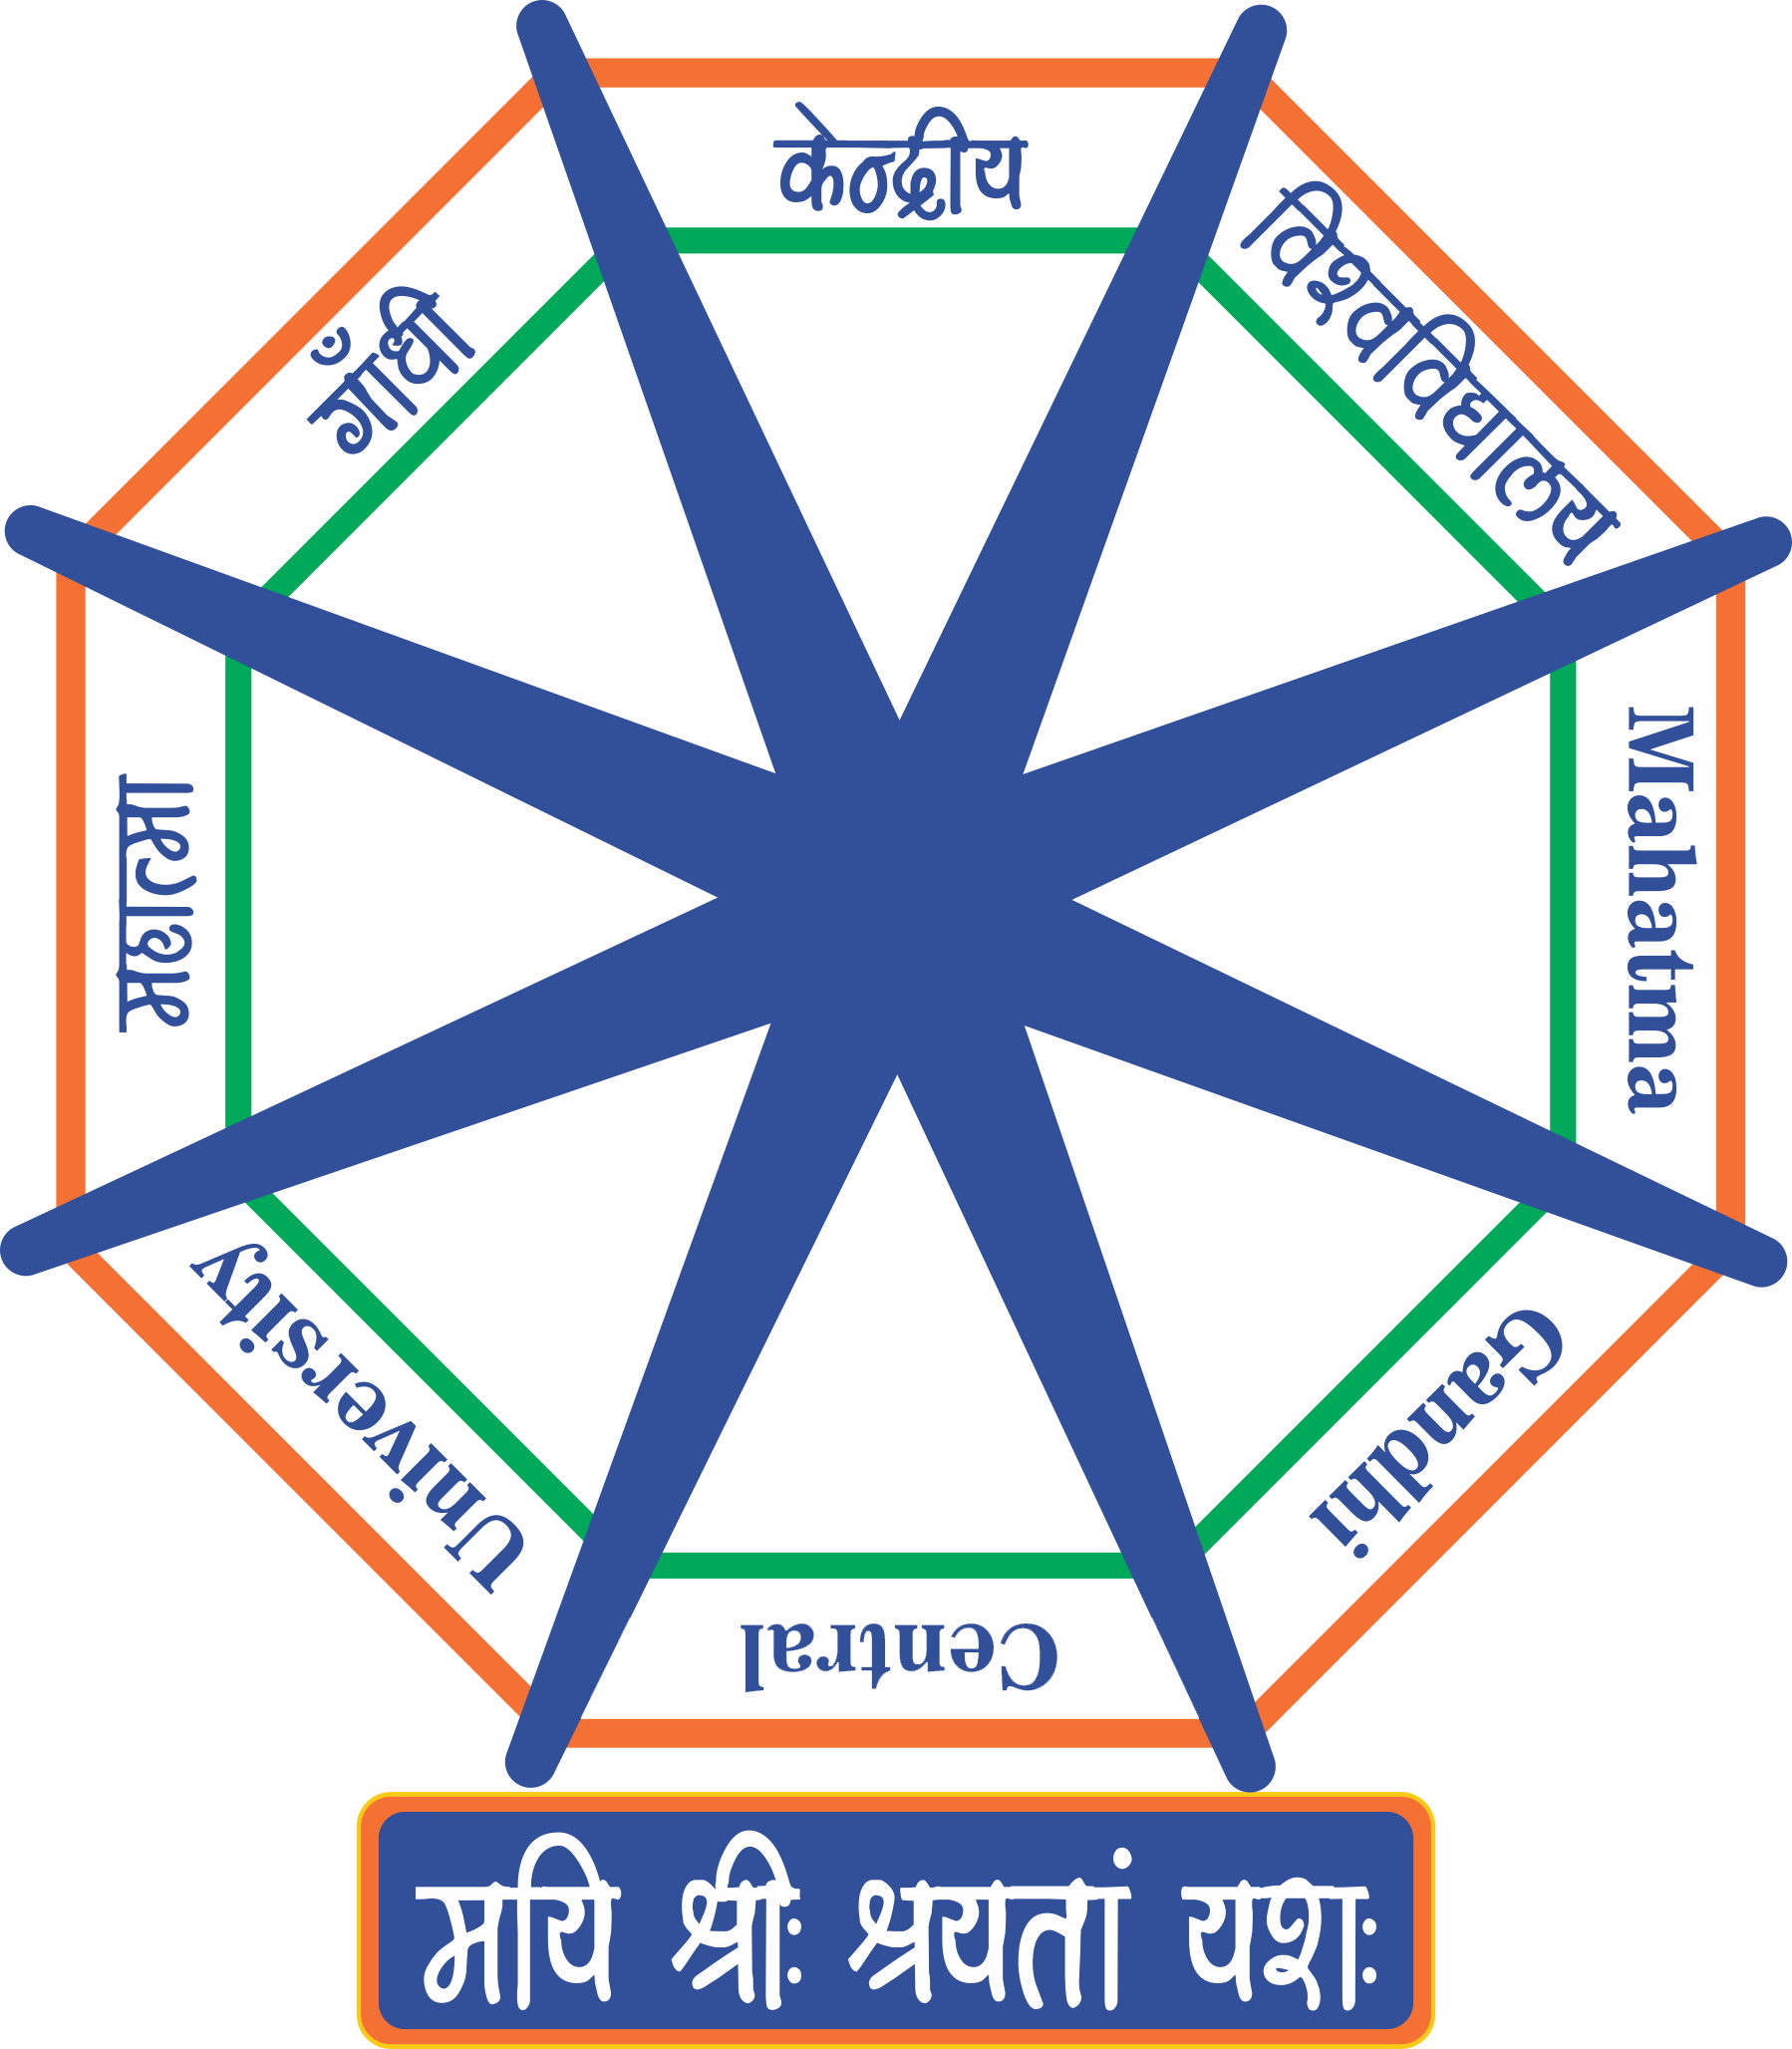
\includegraphics[width=1\textwidth]{mgcu}
    \caption{Actual vs Predicted of BiLSTM for All Datasets}
    \label{img:bilstn_a_p}
\end{figure}
 % Chapter 5
% Chapter Template

\chapter{Conclusion} % Main chapter title

\label{c6} % Change X to a consecutive number; for referencing this chapter elsewhere, use \ref{ChapterX}

\section{Conclusion}

 % Chapter 6
% Back matter

\clearpage \phantomsection \addcontentsline{toc}{chapter}{References} % Add to TOC
\bibliographystyle{plainnat} % Bibliography style
\bibliography{backmatter/mybib} % Bibliography file


\clearpage
\phantomsection
\onehalfspacing
\begin{appendices} 
%%================app1======================================
\chapter{Supporting Information}\label{app:app1}

\begin{figure}[h]
	\centering
	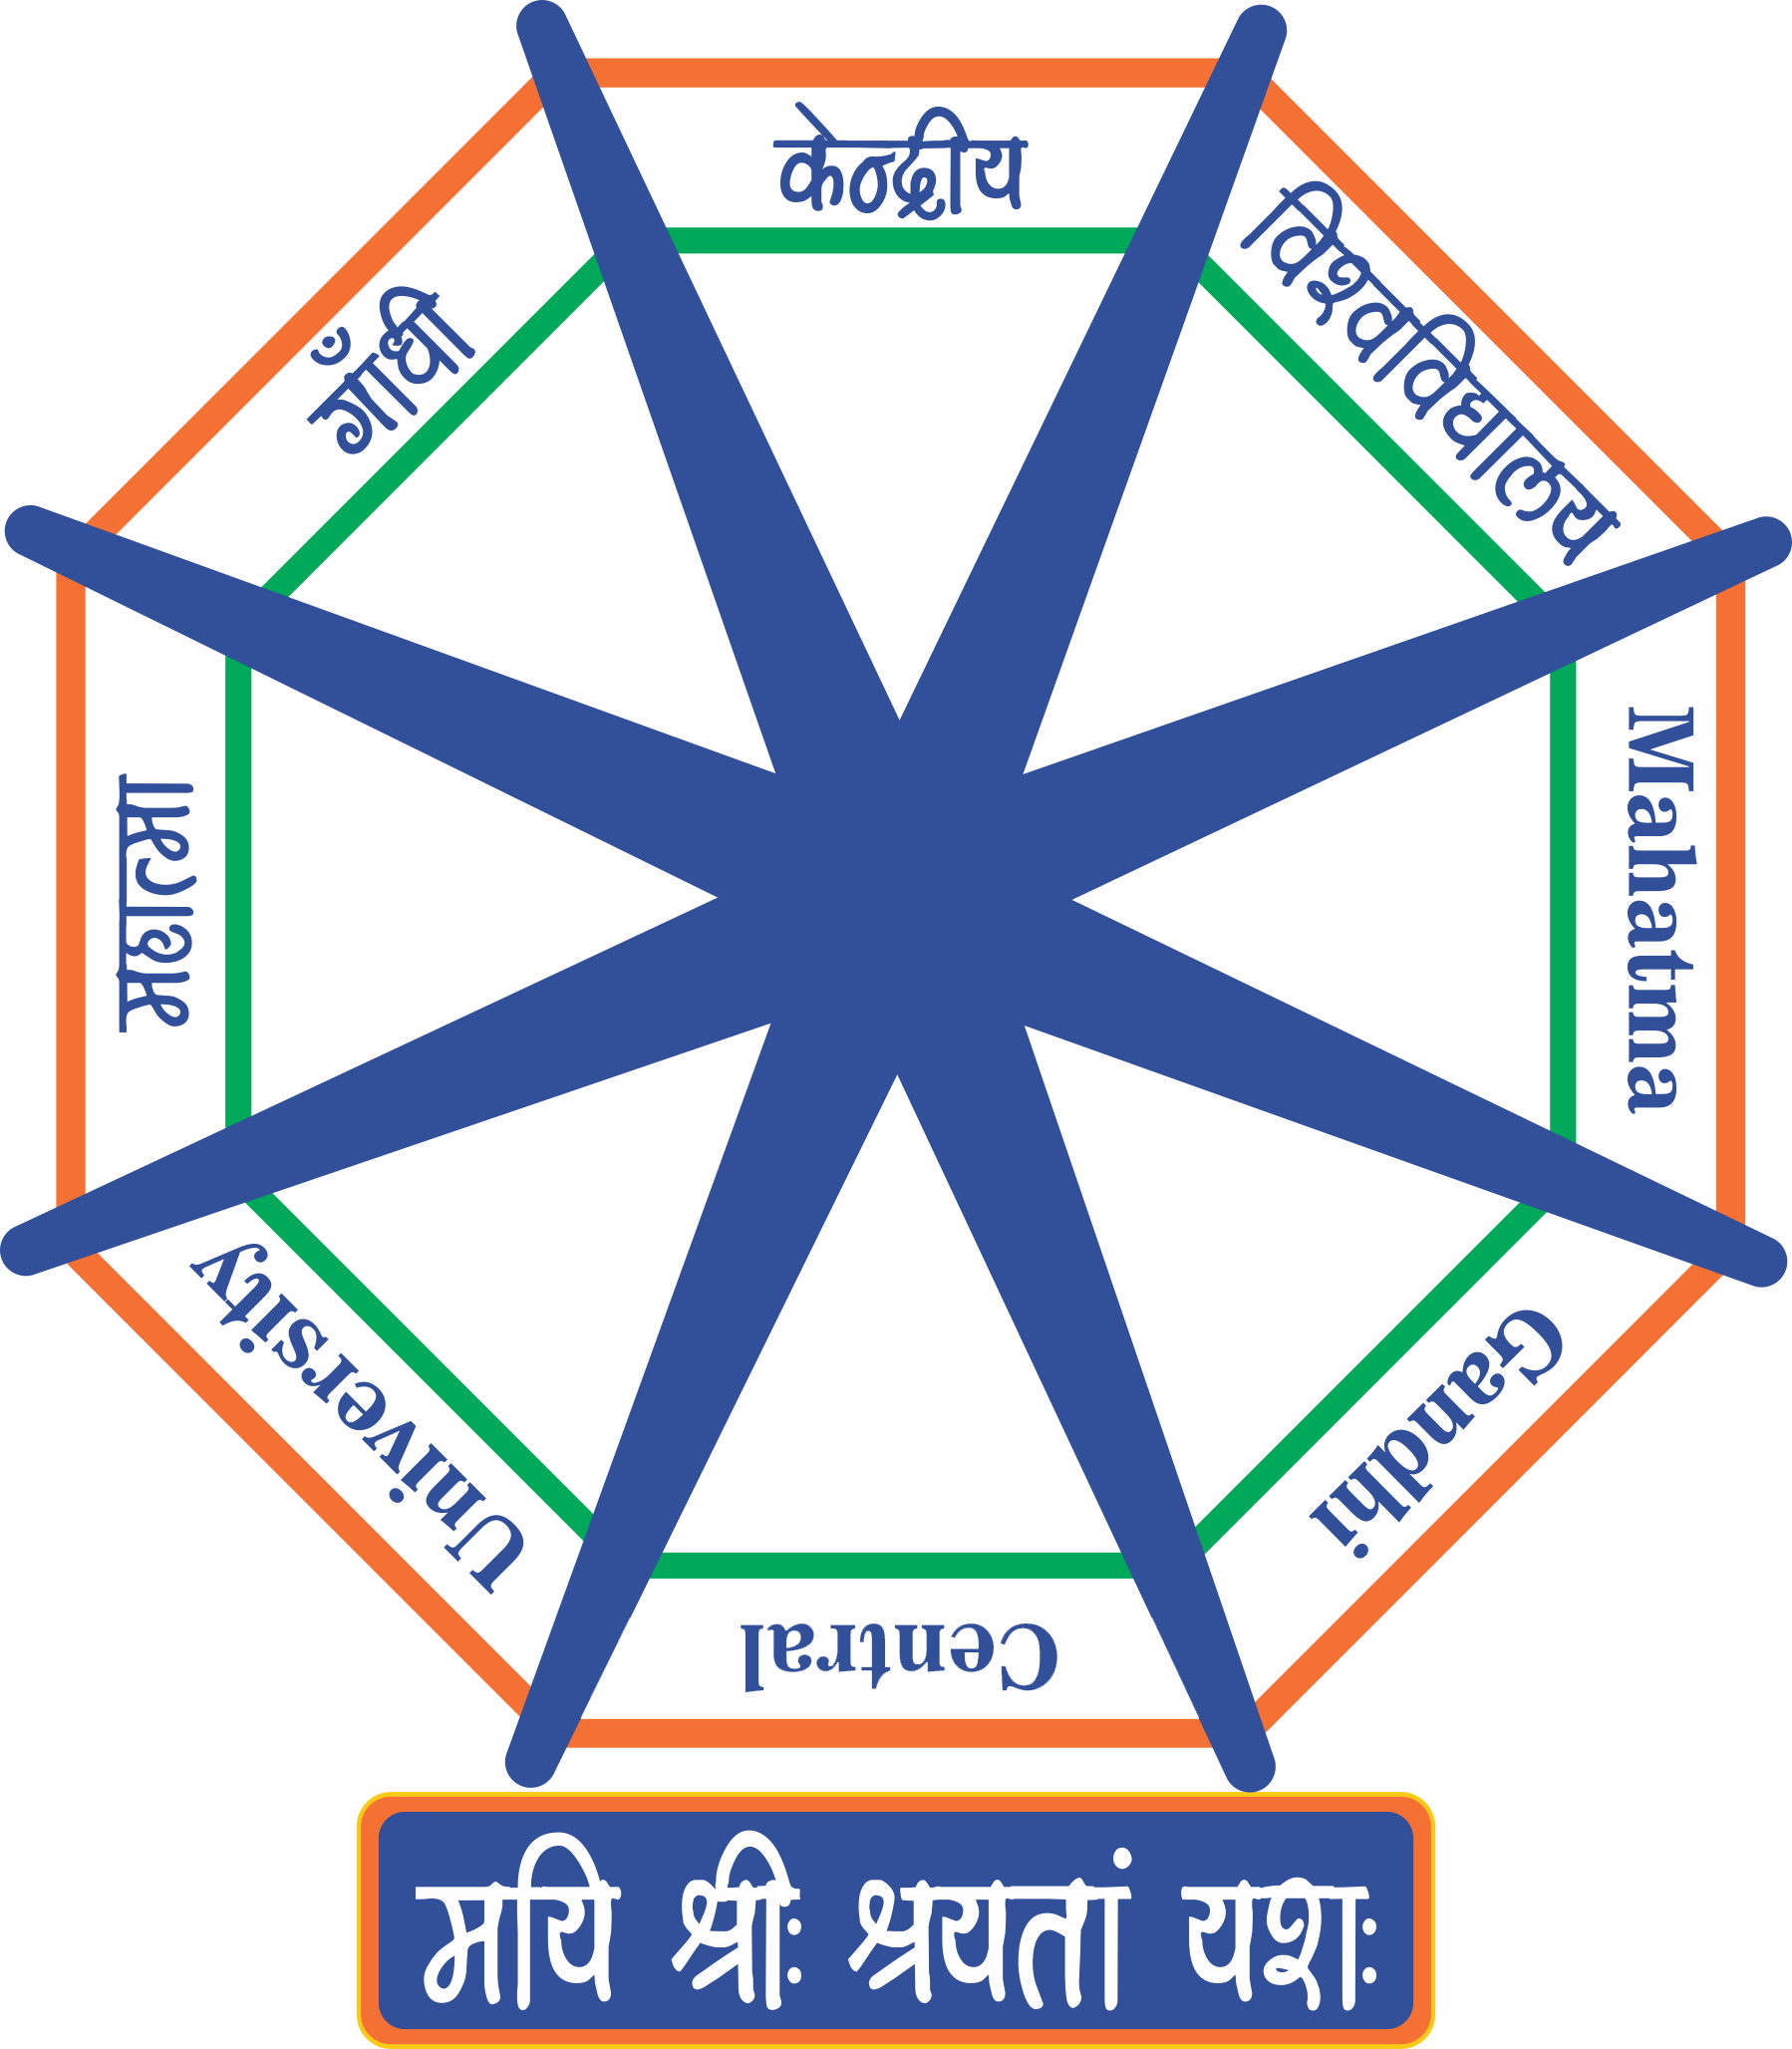
\includegraphics[width=.5\textwidth]{mgcu}
	\caption{Caption of image 2.}
	\label{fig: img2}
\end{figure} % Appendix 1 
%%================app1======================================
\chapter{Supporting Information}\label{app:app2}

\begin{figure}[h]
	\centering
	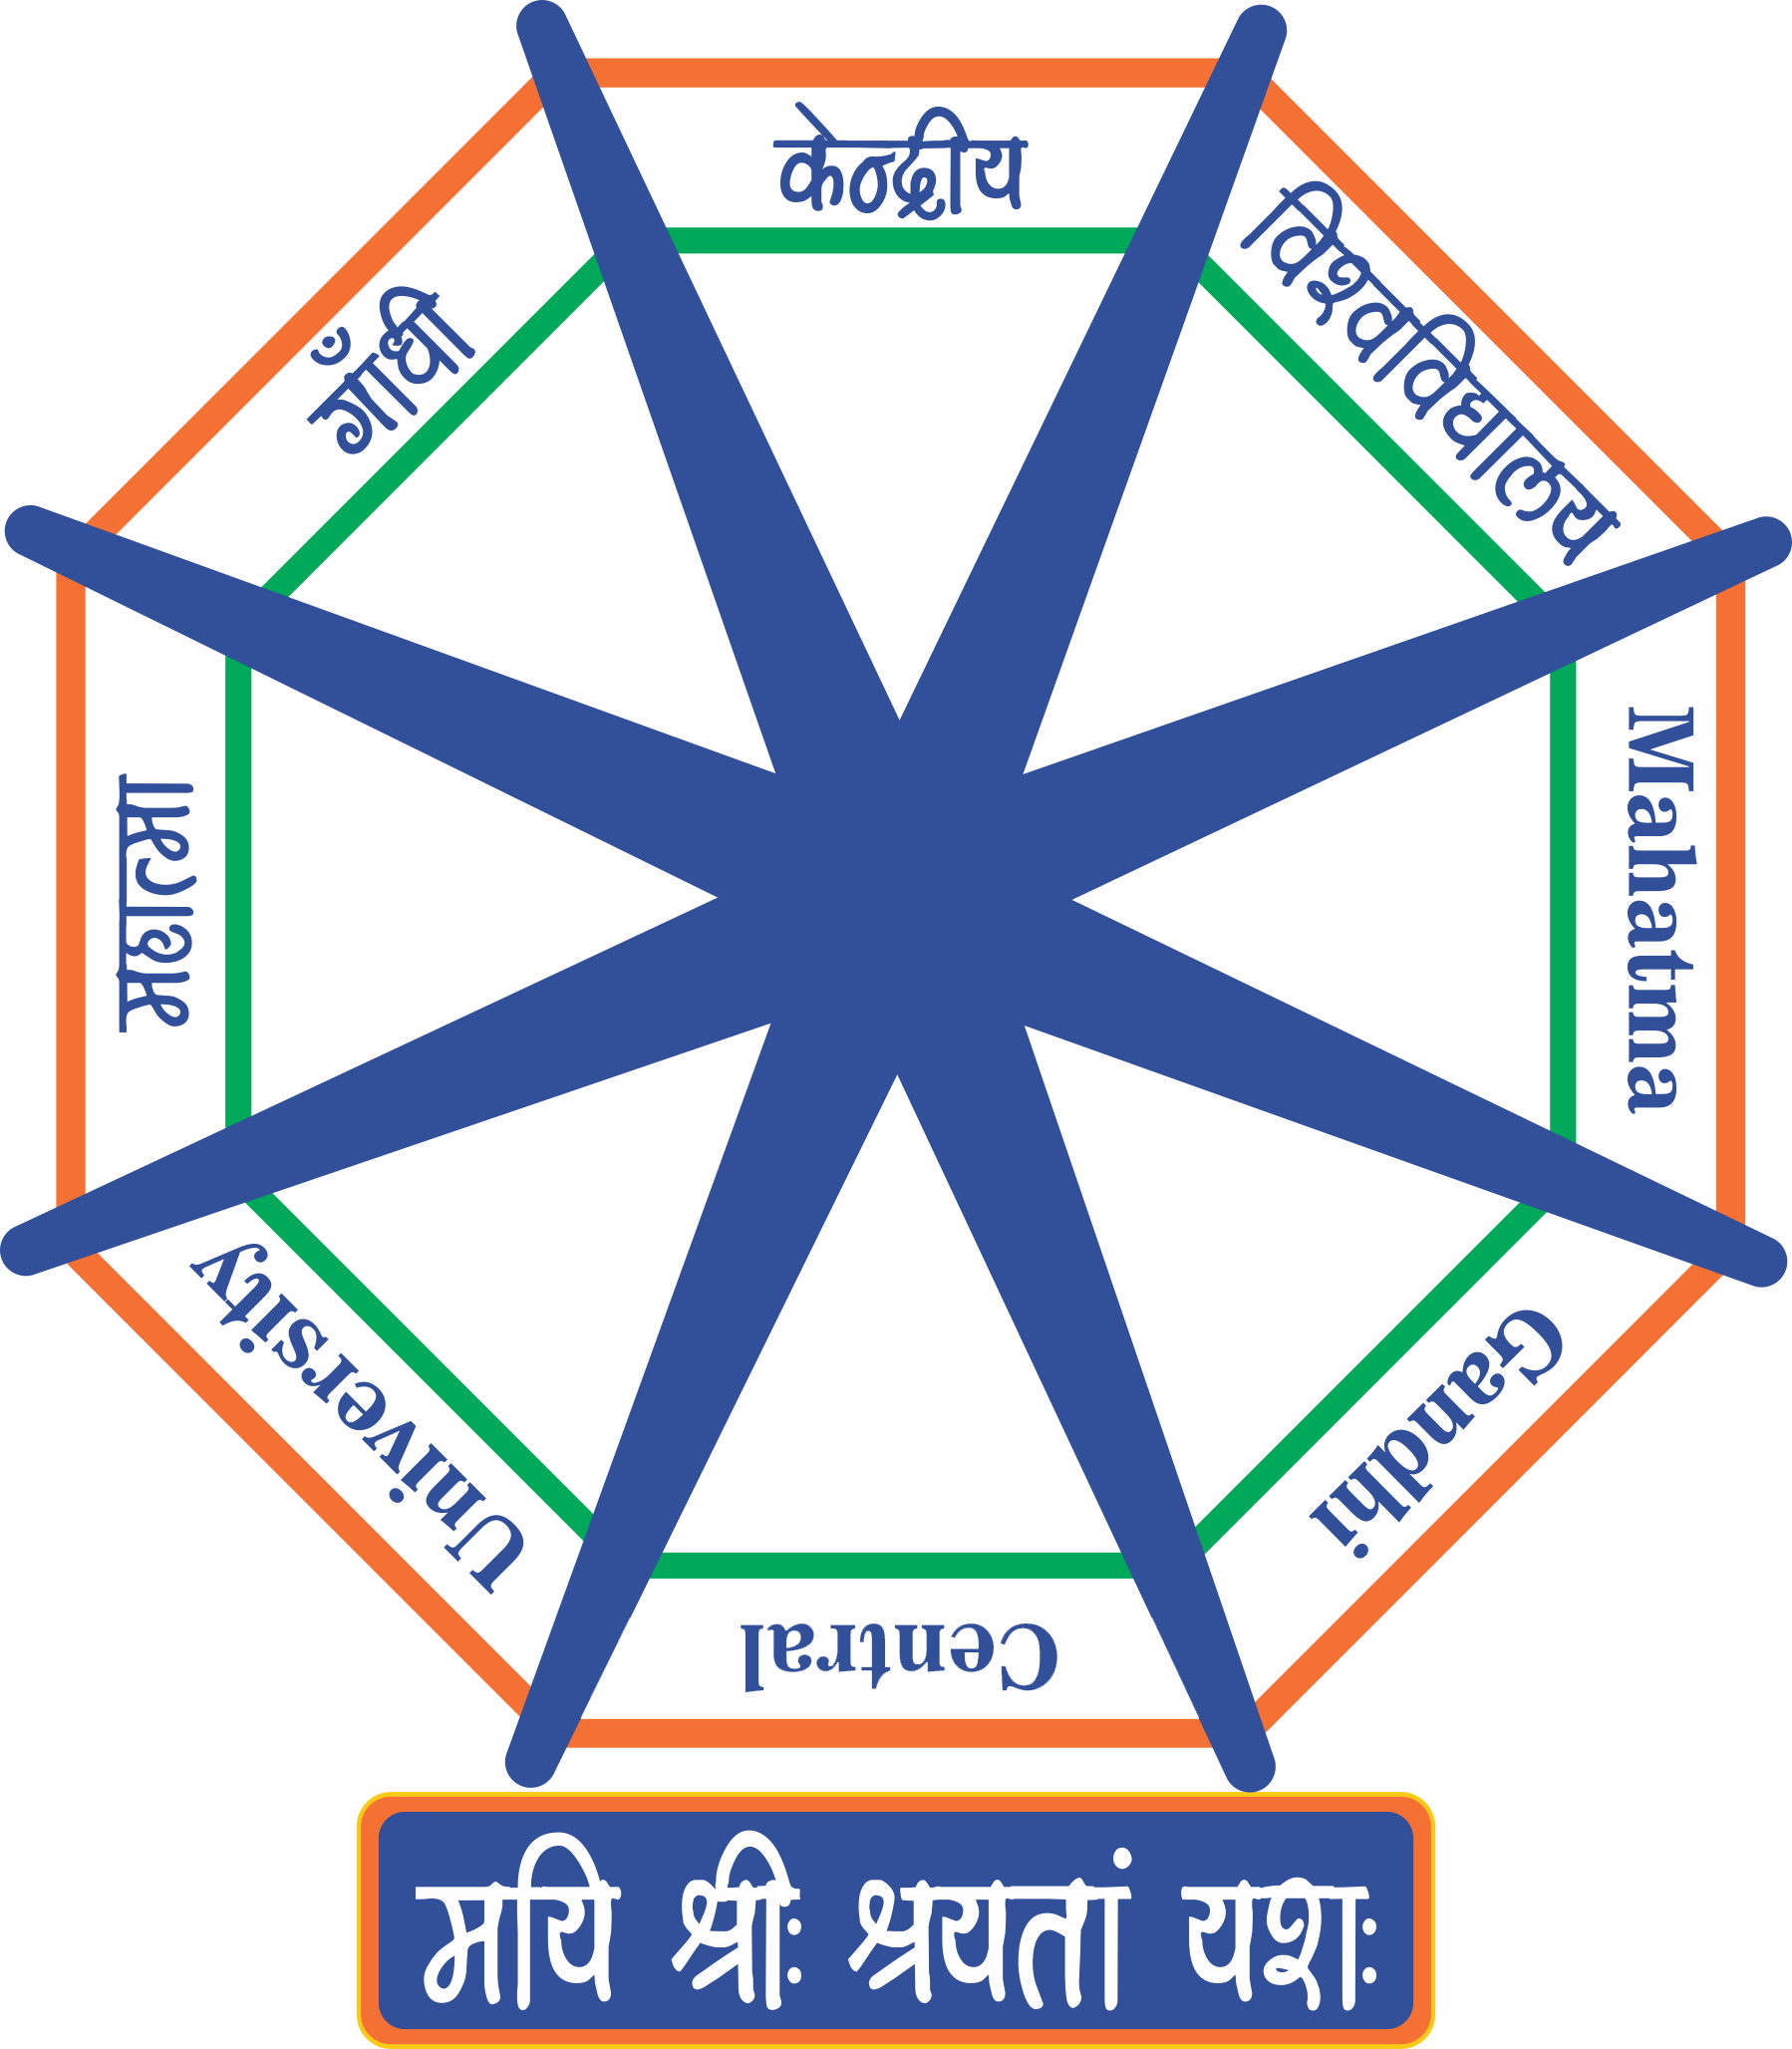
\includegraphics[width=.5\textwidth]{mgcu}
	\caption{Caption of image 2.}
	\label{fig: img2}
\end{figure} % Appendix 2 
\end{appendices} 
%============================= pub.tex================================
\chapter*{List of Publications and Presentations}
\addcontentsline{toc}{chapter}{List of Publications}
	
\section*{Refereed Journals/Manuscripts Under Preparation}
\begin{enumerate}  
  \item A. Autohr, and B. Author. Article title, \textit{Journal Name}, year, \textbf{vol.}, xxxx--xxxx.   
\end{enumerate}

\section*{Book}	
\begin{enumerate}
\item A. Autohr, \textit{Book title}, Under preparation. 
\end{enumerate}

\section*{Conference Abstracts/Posters/Presentations}
\begin{enumerate}
   \item A. Autohr, B. Author, and C.D. Author, Title of the talk/poster, \textit{Conference Name}, Place, Country, day month year.  

   \item A. Autohr, B. Author, and C.D. Author, Title of the talk/poster, \textit{Conference Name}, Place, Country, day month year.      
\end{enumerate}
 % Publications 




\end{document}
